\documentclass{article}

\usepackage{geometry}
\usepackage{amsmath}
\usepackage{graphicx}
\usepackage{listings}
\usepackage{hyperref}
\usepackage{multicol}
\usepackage{fancyhdr}
\pagestyle{fancy}
\hypersetup{ colorlinks=true, linkcolor=black, filecolor=magenta, urlcolor=cyan}
\geometry{ a4paper, total={170mm,257mm}, top=20mm, right=20mm, bottom=20mm, left=20mm}
\setlength{\parindent}{0pt}
\setlength{\parskip}{1em}
\renewcommand{\headrulewidth}{0pt}
\lhead{Competitive Programming - Arkavidia VI}
\fancyfoot[CE,CO]{\thepage}
\lstset{
    basicstyle=\ttfamily\small,
    columns=fixed,
    extendedchars=true,
    breaklines=true,
    tabsize=2,
    prebreak=\raisebox{0ex}[0ex][0ex]{\ensuremath{\hookleftarrow}},
    frame=none,
    showtabs=false,
    showspaces=false,
    showstringspaces=false,
    prebreak={},
    keywordstyle=\color[rgb]{0.627,0.126,0.941},
    commentstyle=\color[rgb]{0.133,0.545,0.133},
    stringstyle=\color[rgb]{01,0,0},
    captionpos=t,
    escapeinside={(\%}{\%)}
}

\begin{document}

\begin{center}
    \section*{Nonogram} % ganti judul soal

    \begin{tabular}{ | c c | }
        \hline
        Batas Waktu  & 1s \\    % jangan lupa ganti time limit
        Batas Memori & 64MB \\  % jangan lupa ganti memory limit
        \hline
    \end{tabular}
\end{center}

\subsection*{Deskripsi}

\textit{Nonogram} atau \textit{Picross} adalah sebuah \textit{game} yang dimainkan pada sebuah papan dua dimensi.
Pada setiap baris dan kolomnya akan terdapat suatu deretan bilangan.
Setiap bilangan pada deretan bilangan tersebut menunjukkan banyak sel bersebelahan 
yang terisi pada baris atau kolom tersebut. Deretan sel terisi pada suatu baris maupun kolom tidak 
dapat menempel dengan deretan sel terisi lainnya

Berikut contoh dari sebuah papan \textit{Nonogram}.

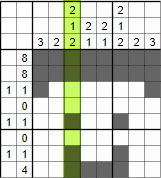
\includegraphics[width=100px]{Nonogram-Steve}

\texit{Game} \textit{Nonogram} akan selesai dimainkan apabila konfigurasi deretan sel yang terisi 
sesuai dengan deretan angka yang ada di setiap baris dan kolom.

Nana sekarang sedang bermain \textit{Nonogram}. Karena Nana tidak punya banyak waktu, 
Nana hanya akan bermain \textit{Nonogram} yang ukurannya $1$ x $N$ (Hanya memiliki $1$ baris dan $N$ kolom). 
Nana sudah berhasil mengisi beberapa sel pada papan \textit{Nonogram}nya, Nana sekarang malah penasaran ada 
berapa banyak cara pengisian sel yang masih kosong sehingga permainan \textit{Nonogram}nya dapat selesai. Sebagai teman baik Nana, dapatkah Anda membantu Nana?


\subsection*{Format Masukan}

Baris pertama terdiri dari satu bilangan bulat positif $N$ ($1 \leq N \leq 5000$), yaitu ukuran kolom papan \textit{Nonogram} yang sedang dimainkan Nana.
Baris berikutnya berisi $N$ bilangan dengan nilai 0 atau 1 yang mendeskripsikan kondisi papan \texit{Nonogram} yang sedang dimainkan Nana. 
Nilai 0 mengindikasikan sel yang masih kosong dan 1 mengindikasikan sel yang sudah terisi.
Baris berikutnya berisi satu bilangan bulat positif $K$ ($1 \leq K \leq 5000$), yaitu banyak bilangan pada deretan bilangan yang sesuai dengan baris pada papan \textit{Nonogram}.
Baris berikutnya berisi $K$ bilangan bulat positif $B$ ($1 \leq B \leq 5000$) yang menunjukkan banyak sel yang terisi pada satu deretan.

Contoh:

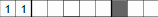
\includegraphics[width=100px]{Nonogram-Row}

Pada gambar tersebut, $N$ bernilai 8 dengan deretan nilai [0, 0, 0, 0, 0, 1, 0, 0], dan $K$ bernilai 2 dengan nilai [1, 1].

\subsection*{Format Keluaran}

Keluarkan sebuah bilangan yang merupakan banyaknya konfigurasi pengisian sel-sel yang masih kosong pada \texit{Nonogram} 
sehingga permainan tersebut selesai dimodulo dengan $10^{9}+7$
\\

\begin{multicols}{2}
\subsection*{Contoh Masukan}
\begin{lstlisting}
8
0 0 0 0 0 1 0 0
2
1 1
\end{lstlisting}
\columnbreak
\subsection*{Contoh Keluaran}
\begin{lstlisting}
5
\end{lstlisting}
\vfill
\null
\end{multicols}

\pagebreak

\end{document}
